\documentclass[10pt]{article}

% The following command leaves more space between lines.  That's great
% when correcting drafts.  When you comment it out, however, the
% output looks much nicer.
%
\linespread{1.0}

\usepackage{amsmath}
\usepackage{amssymb}
\usepackage{graphicx}
\usepackage{epsfig}
\usepackage{latexsym}
\usepackage{amsthm}

\usepackage{mathrsfs}

\usepackage{multicol}



\usepackage[colorlinks,citecolor=blue]{hyperref}

\usepackage[latin1]{inputenc}

\usepackage{tikz-cd}
\usepackage{pgfplots}

%\usepackage{3dplot}

\usetikzlibrary{matrix,arrows,decorations.pathmorphing}


\usepackage[scale=0.8]{geometry}


%\usepackage{umoline}\setlength{\UnderlineDepth}{1pt}
%\usepackage[linktocpage=true]{hyperref}

\input xy
\xyoption{all}


%\addtolength{\hoffset}{-.5in}
%\addtolength{\textwidth}{1in}
%\setlength{\parindent}{.5in}
%\setlength{\textheight}{9.5in} \setlength{\topmargin}{-2cm}


\pagestyle{myheadings}\parindent 0em




\usepackage[latin1]{inputenc}


%------------------copy and posted code from the internets-------------

%\numberwithin{equation}{section} % comment out when neccessary

\newtheorem{theorem}[equation]{Theorem}
\newtheorem{lemma}[equation]{Lemma}
\newtheorem{proposition}[equation]{Proposition}
\newtheorem{corollary}[equation]{Corollary}


\theoremstyle{definition}
\newtheorem{definition}[equation]{Definition}
\newtheorem{example}[equation]{Example}
\newtheorem{remark}[equation]{Remark}
\newtheorem{problem}[equation]{Problem}



\newcommand{\R}[1]{\mathbb{R}^{#1}}
\newcommand{\C}[1]{\mathbb{C}^{#1}}
\newcommand{\Z}[1]{\mathbb{Z}^{#1}}
\newcommand{\K}[1]{\mathbb{K}^{#1}}
\newcommand{\embed}[0]{\hookrightarrow}
\newcommand{\TT}[4]{\begin{tabular}{| c | c |}\hline $#1$ & $#2$ \\ \hline $#3$ & $#4$ \\ \hline\end{tabular}} %goddamn it
\newcommand{\partd}[2]{\frac{\partial #1}{\partial #2}}
\newcommand{\limit}[2]{\displaystyle{ \lim_{#1 \to #2}}}
\newcommand{\vectornorm}[1]{\left|\left|#1\right|\right|}
\newcommand{\Ker}[0]{\text{\textnormal{Ker}}}
\newcommand{\Hom}[0]{\text{\textnormal{Hom}}}
\newcommand{\circled}[1]{\tikz[baseline=(char.base)]{
            \node[shape=circle,draw,inner sep=2pt] (char) {#1};}}


\newcommand{\T}{\rotatebox[origin=c]{180}{$\scriptscriptstyle \perp $}}
\newcommand{\x}{\textbf{x}}
\newcommand{\y}{\textbf{y}}
\newcommand{\supp}{\text{\textnormal{supp}}}
\newcommand{\csupp}{\text{\textnormal{cosupp}}}
\newcommand{\found}{\text{\textnormal{found}}}
\newcommand{\roof}{\text{\textnormal{roof}}}

\newcommand{\bcup}{\displaystyle\bigcup}
\newcommand{\bcap}{\displaystyle\bigcap}
\newcommand{\dsum}{\displaystyle\sum}
\newcommand{\dint}{\displaystyle\int}





\begin{document}
%

{\bf Name:} \hrulefill\hrulefill\hrulefill\\
{\bf Stat-216} \qquad \qquad \\
{\bf Linear Regression }\\ %(look familiar??)\\
%Show all work for full/partial credit.
%---------------- End of the document ---------------



\section{Philosophy of Linear Regression}

It turns out that it's fairly rare to find variables in the world that are truly independent of each other.  The world is full of variables that have hidden connections and part of understanding the universe we exist in is uncovering all these connections.  This is true since the first cave person stood near a fire and realized that standing near a fire made them warmer, thus uncovering a connection between standing near fires and warmth.\\

However, since the world is an interconnected web of hidden influences, it's rare to see two variables that can be solely and completely determined by one another.  In the example of our erstwhile caveperson, it's certain that standing near fire could make you warm, but so could standing in sunlight, so could wearing more furs.  There are a lot of factors that go into determining warmth besides proximity to flames.\\

Our goal here then is to take observations and determine whether or not they are connected, and what the connection is so we could potentially use one as a predictor for the other.  But moreover, we also want to measure how strong this connection is so that we can asses how accurate these predictions might be, and what other variables may be influencing these outcomes.


\section{Basic Mechanics of Linear Regression}

Consider the data set:

$$\begin{array}{c|c}
x&y\\
\hline
1&2\\
2&2\\
3&4\\
4&4\\
5&6
\end{array}$$


If we were to plot this data, it would look like:

$$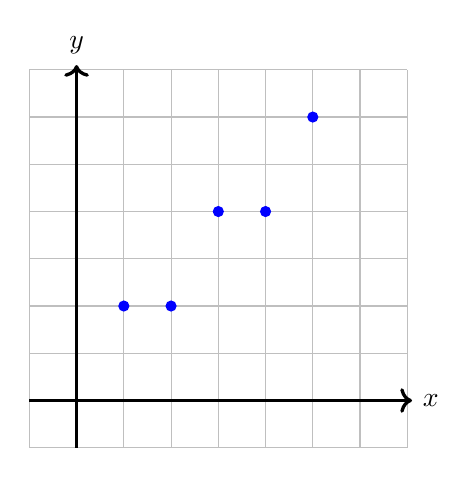
\begin{tikzpicture}[scale=.6][domain=-1:7]
    \draw[gray!50, thin, step=1] (-1,-1) grid (7,7);
    \draw[very thick,->] (-1,0) -- (7.1,0) node[right] {$x$};
    \draw[very thick,->] (0,-1) -- (0,7.1) node[above] {$y$};

%    \foreach \x in {-4,...,10} \draw (\x,0.05) -- (\x,-0.05) node[below] {\tiny\x};
%    \foreach \y in {-2,...,2} \draw (-0.05,\y) -- (0.05,\y) node[right] {\tiny\y};

\draw[blue, fill] (1,2) circle (3pt);
\draw[blue, fill] (2,2) circle (3pt);
\draw[blue, fill] (3,4) circle (3pt);
\draw[blue, fill] (4,4) circle (3pt);
\draw[blue, fill] (5,6) circle (3pt);

%  \draw[scale=1,domain=-2:2,smooth,variable=\x,blue] plot ({\x},{\x*\x*\x-3*\x}) node[above]{$y=f(x)$};


\end{tikzpicture}$$ % of mbox

Our goal here is to find a linear relationship between $x$ and $y$.  Graphically that means we want to draw a line that best fits the data we present here.  Of course, there is no line that can pass through all these points.  So our goal is to find a line that minimizes the error or ``residuals" that would arise as a result.  Part of the condition of being a regression line is that the sum of these errors should be zero.

So we define the following:

\begin{itemize}
\item $SS_X=\sum(x_i-\bar{x})^2=\sum x_i^2-\frac{(\sum x_i)^2}{n}$
\item $SS_Y=\sum(y_i-\bar{y})^2=\sum y_i^2-\frac{(\sum y_i)^2}{n}$
\item $SS_{XY}=\sum(x_i-\bar{x})(y_i-\bar{y})=\sum x_iy_i-\frac{(\sum x_i)(\sum y_i)}{n}$
\end{itemize}

Where $SS$ stands for ``Sum of Squares".  We see that this is reminiscent of the standard deviation formulas.  Then the slope of the regression line will be:

$$\beta_1:=\frac{SS_{XY}}{SS_{X}}$$

If we recall, a line needs not just a slope, but a $y$ intercept.  So how can we figure out what the $y$ intercept should be?  Well, given the slope $\beta_1$, ON AVERAGE, given some $x_i$, we should get that $y_i=\beta_1x_i+\beta_0$, where $\beta_0$ is our yet-unknown $y$-intercept.  Again, this won't happen every time, or possibly ever, but it should be the average result, so the way we find $\beta_0$ is:

\begin{eqnarray*}
\bar{y}&=&\beta_1\bar{x}+\beta_0\\
\beta_0&=&\bar{y}-\beta_1\bar{x}.
\end{eqnarray*}

So for our example data:

\begin{eqnarray*}
\bar{x}&=&\frac{1+2+3+4+5}{5}=3\\
\bar{y}&=&\frac{2+2+4+4+6}{5}=3.6\\
SS_X&=&(1-3)^2+(2-3)^2+(3-3)^2+(4-3)^2+(5-3)^2=10\\
SS_Y&=&(2-3.5)^2+(2-3.5)^2+(4-3.5)^2+(4-3.5)^2+(6-3.5)^2=11.25\\
SS_{XY}&=&(1-3)(2-3.5)+(2-3)(2-3.5)+(3-3)(4-3.5)+(4-3)(4-3.5)+(5-3)(6-3.5)=10\\
\beta_1&=&\frac{10}{10}=1\\
\beta_0&=&3.6-(1)(3)=0.6
\end{eqnarray*}

So our best fit line is $y=1x+0.6$.



$$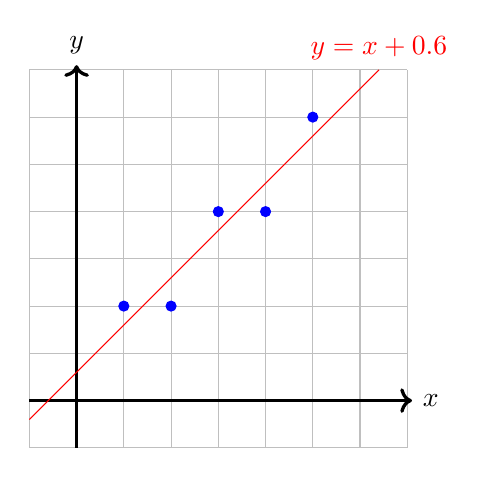
\begin{tikzpicture}[scale=.6][domain=-1:7]
    \draw[gray!50, thin, step=1] (-1,-1) grid (7,7);
    \draw[very thick,->] (-1,0) -- (7.1,0) node[right] {$x$};
    \draw[very thick,->] (0,-1) -- (0,7.1) node[above] {$y$};

%    \foreach \x in {-4,...,10} \draw (\x,0.05) -- (\x,-0.05) node[below] {\tiny\x};
%    \foreach \y in {-2,...,2} \draw (-0.05,\y) -- (0.05,\y) node[right] {\tiny\y};

\draw[blue, fill] (1,2) circle (3pt);
\draw[blue, fill] (2,2) circle (3pt);
\draw[blue, fill] (3,4) circle (3pt);
\draw[blue, fill] (4,4) circle (3pt);
\draw[blue, fill] (5,6) circle (3pt);

  \draw[scale=1,domain=-1:6.4,smooth,variable=\x,red] plot ({\x},{\x+0.6}) node[above]{$y=x+0.6$};


\end{tikzpicture}$$

Again, notice that none of the points actually fall on this line, but no possible line could have accomplished all of the points falling on it.  What we have instead is a line that passes through the points as closely as possible.  Define $e_i$ to be the error in prediction for $y_i$, that is let $e_i=y_i-(1\cdot x_i+0.6)$, then we see that:

\begin{eqnarray*}
e_1&=&2-(1+.6)=0.4\\
e_2&=&2-(2+.6)=-0.6\\
e_3&=&4-(3+.6)=0.4\\
e_4&=&4-(4+.6)=-0.6\\
e_5&=&6-(5+.6)=0.4
\end{eqnarray*}

$$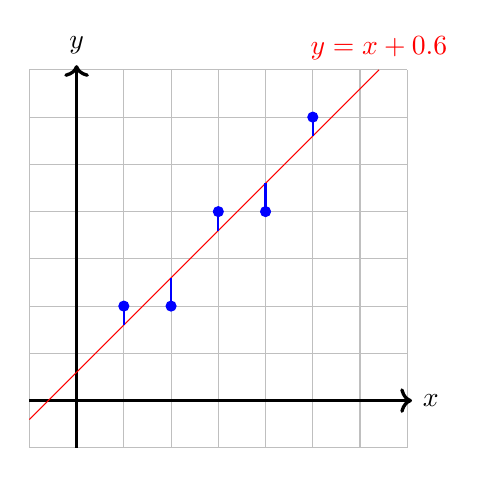
\begin{tikzpicture}[scale=.6][domain=-1:7]
    \draw[gray!50, thin, step=1] (-1,-1) grid (7,7);
    \draw[very thick,->] (-1,0) -- (7.1,0) node[right] {$x$};
    \draw[very thick,->] (0,-1) -- (0,7.1) node[above] {$y$};

%    \foreach \x in {-4,...,10} \draw (\x,0.05) -- (\x,-0.05) node[below] {\tiny\x};
%    \foreach \y in {-2,...,2} \draw (-0.05,\y) -- (0.05,\y) node[right] {\tiny\y};

\draw[blue, fill] (1,2) circle (3pt);
\draw[blue, fill] (2,2) circle (3pt);
\draw[blue, fill] (3,4) circle (3pt);
\draw[blue, fill] (4,4) circle (3pt);
\draw[blue, fill] (5,6) circle (3pt);

  \draw[scale=1,domain=-1:6.4,smooth,variable=\x,red] plot ({\x},{\x+0.6}) node[above]{$y=x+0.6$};

\draw[blue, thick](1, 1.6) -- (1,2);
\draw[blue, thick](2, 2.6) -- (2,2);
\draw[blue, thick](3, 3.6) -- (3,4);
\draw[blue, thick](4, 4.6) -- (4,4);
\draw[blue, thick](5, 5.6) -- (5,6);


\end{tikzpicture}$$


But $$e_1+e_2+e_3+e_4+e_5=(0.4)+(-0.6)+(0.4)+(0.6)+(0.4)=0.$$


{\bf WHAT DOES THIS MEAN?} That means if we wanted to predict what would happen when $x=7$ or $x=10$, we could  plug in 7 or 10 into $y=x+0.6$ and be reasonably assured that the actual associated $y$ value would be close to that.


{\bf THIS WAS A LOT OF WORK JUST TO FIND A LINE, ISN'T THERE AN EASIER WAY?}   There sure is: \url{https://www.desmos.com/calculator/tfoo1bme8u}\\


We notice that when we evaluate this in desmos, we are also given a correlation coefficient $r=0.9449$, and it's square $r^2=0.8929$.  These coefficients measure the following:

\begin{itemize}
\item $r$ measures whether or not the correlation is a positive or negative one.  It in effect determines whether or not the slope of the best fit line is positive or negative.
\item $r^2$ measure the strength of the connection between $x$ and $y$, the closer to 1, the stronger the connection.
\end{itemize}

So in this case $r=0.9449$ means that the correlation is a positive one, and $r^2=0.8929$ means that $y$ is roughly 89.29\% predictable by $x$ and 10.71\% determined by other factors, so it's fairly strong.\\

We do one more example before applying this to real situations:\\

  Consider the following data:



$$\begin{array}{c|c}
x&y\\
\hline
1&1\\
1&2\\
2&1\\
2&2\\
3&1\\
3&2
\end{array}$$


When we plot this, it looks like:

$$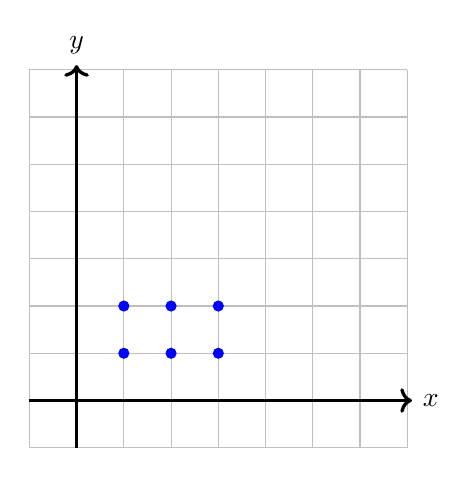
\begin{tikzpicture}[scale=.6][domain=-1:7]
    \draw[gray!50, thin, step=1] (-1,-1) grid (7,7);
    \draw[very thick,->] (-1,0) -- (7.1,0) node[right] {$x$};
    \draw[very thick,->] (0,-1) -- (0,7.1) node[above] {$y$};

%    \foreach \x in {-4,...,10} \draw (\x,0.05) -- (\x,-0.05) node[below] {\tiny\x};
%    \foreach \y in {-2,...,2} \draw (-0.05,\y) -- (0.05,\y) node[right] {\tiny\y};

\draw[blue, fill] (1,1) circle (3pt);
\draw[blue, fill] (1,2) circle (3pt);
\draw[blue, fill] (2,1) circle (3pt);
\draw[blue, fill] (2,2) circle (3pt);
\draw[blue, fill] (3,1) circle (3pt);
\draw[blue, fill] (3,2) circle (3pt);

%  \draw[scale=1,domain=-2:2,smooth,variable=\x,blue] plot ({\x},{\x*\x*\x-3*\x}) node[above]{$y=f(x)$};


\end{tikzpicture}$$ % of mbox

What our intuition should tell us is that it doesn't seem like the outputs $y$ change at all given changes in $x$.  So here, we may in fact see that $y$'s outputs are completely independent of $x's$.  This would mean that there is NO correlation between $x$ and $y$ and sure enough: \url{https://www.desmos.com/calculator/pcwpzyrjc4}, we observe that $r, r^2=0$.  This means that no part of $y$ is determined by $x$.


\section{Applications}

\begin{example}
From fbi.gov from 2004-2013, the murder rates per 100,000 people are listed below:

$$\begin{array}{c|c}
\text{Years after 2000} & \text{Murders per 100,000 people}\\
x&y\\
\hline
4&5.5\\
5&5.6\\
6&5.8\\
7&5.7\\
8&5.4\\
9&5\\
10&4.8\\
11&4.7\\
12&4.7\\
13&4.5
\end{array}$$
\begin{enumerate}
\item Determine the best fit line for murders (per 100,000 people) $x$ years after 2000.
\item How much of a factor is the year in predictiung the number of murders?
\item Predict the murder rate in 2018.
\end{enumerate}

Entering this data in desmos: \url{https://www.desmos.com/calculator/em6xkq7udn}

\begin{enumerate}
\item It seems that the best fit line is $y=-0.144848x+6.40121$.
\item Since $r^2=0.8318$, we can say the murder rate is 83.18\% predictable by the year.
\item In 2018, the murder rate should be $-0.144848(18)+6.40121=3.793946$ or roughly 3.8 murders per 100,000 people in 2018.
\end{enumerate}




\end{example}



\begin{example}
I personally wondered in quiz scores are a good predictor of test scores in Calculus.  I pulled out some data from this semester, and here are the average quiz and test scores of my students, anonymously of course:


$$\begin{array}{c|c}
\text{Quiz Average} & \text{Test Average}\\
x&y\\
\hline
87.5&100\\
76.13&94\\
75.83&93.5\\
53.53&83.5\\
76.13&83\\
71.13&78.85\\
56.13&76.5\\
73.57&70\\
66.13&69.5\\
66.13&63
\end{array}$$



\end{example}
\begin{enumerate}
\item Find the linear relationship between Quiz grades and Test grades.
\item Are Quiz grades a good predictor of Test grades?
\item If someone has an 80 average on Quizzes, predict their Test grade.
\end{enumerate}

So, once again:  \url{https://www.desmos.com/calculator/atipunytb1}

\begin{enumerate}
\item The relationship here is: $y=0.639883x+36.2168$, so there is a positive correlation, which we expect.
\item $r^2=0.2906$, so Test grades 29.06\% predictable by Quiz grades, which one would also expect, some people perform better in the Exam situation and some people perform worse.
\item We would have an expected test grade of $y=0.639883(80)+36.2168=87.40744$ or about 87.41\%.  But of course with an $r^2$ that small we shouldn't expect this to be terribly accurate.
\end{enumerate}












\end{document}
